\documentclass[a4paper,9pt]{scrartcl}
\usepackage[nuk]{babel}
\usepackage[utf8]{inputenc}
\usepackage{amssymb,amsmath}
\usepackage{geometry}
\geometry{a4paper,left=18mm,right=18mm, top=2cm, bottom=2cm}

\title{A2 Physics}

\usepackage{lipsum}
\usepackage{ctex}
\usepackage{enumerate}
\usepackage{listings}
\usepackage{graphicx}

\begin{document}

    \section{Circular motion}

    \subsection{Circular acceleration}

    \subsubsection{Relations}
    \begin{displaymath}
        a_c = \omega^{2}r = \frac{v^2}{r} = \frac{4\pi^{2}r}{T^{2}} = {\omega}v
    \end{displaymath}

    \begin{displaymath}
        \omega = \frac{2\pi}{T}
    \end{displaymath}

    \begin{displaymath}
        v = {\omega}r = \frac{2{\pi}r}{T}
    \end{displaymath}

    \subsection{Angular velocity}

    \subsubsection{Definition}
    \textit{Angular displacement swept out by radius, per unit time.}


    \section{Gravitational field \& Electric field}

    \subsection{Potential, Force, Energy}

    \subsubsection{Electric Field Strength}
    \begin{displaymath}
        E = \frac{kQ}{r^2}
    \end{displaymath}

    \subsubsection{Electric Potential}
    \begin{displaymath}
        \Phi = \frac{kQ}{r}
    \end{displaymath}

    \subsubsection{Electric Potential Energy}
    \begin{displaymath}
        E_p = \frac{kQq}{r}
    \end{displaymath}

    \subsubsection{Electric Force}
    \begin{displaymath}
        F = \frac{kQq}{r^2}
    \end{displaymath}

    \subsection{Electric field}

    \subsubsection{Definitions}
    \begin{itemize}
        \item~\textbf{A field of force}: \textit{region of space where a particle experiences a force}
    \end{itemize}

    \subsection{Gravitational field}

    \subsubsection{Definition}

    \begin{itemize}
        \item~\textbf{A line of force in a gravitational field}: \textit{Tangent to line gives direction of force on a mass}
        \item~\textbf{A line of force in a electric field}: \textit{Tangent to line gives direction of force on a positive charge}
    \end{itemize}

    \subsubsection{Why gravitational potential is negative}
    \begin{itemize}
        \item gravitational potential at infinity is zero
        \item gravitational force is attractive so work was done as objects move from infinity
    \end{itemize}

    \subsubsection{Difference between gravitation field and electric field}
    \begin{itemize}
        \item Gravitational force always attractive
        \item Electric field forces are attractive or repulsive
    \end{itemize}


    \section{Capacitor}

    \subsection{Capacitor}

    \subsubsection{Function of capacitor}
    \begin{itemize}
        \item Storage of energy
        \item Smoothing
        \item Blocking of direct current
        \item Producing of electrical oscillation
    \end{itemize}

    \subsubsection{Why capacitor stores energy, no charge}
    \begin{itemize}
        \item Positive and negative charges are separated, work done to achieve this, so stores energy
        \item The two plates have equal and opposite charges, so resultant charge is zero
    \end{itemize}

    \subsection{Capacitance}

    \subsubsection{Definition}
    \textit{Charge / Potential difference. [1]}\\
    \textit{The ratio of charge on one plate to the potential difference between plates. [2]}\\
    \begin{displaymath}
        Q = CV
    \end{displaymath}

    \subsubsection{Capacitance is a property}
    \begin{displaymath}
        C = \frac{\epsilon_{0}A}{d}
    \end{displaymath}
    where A is the area of one of the plates, and d is the plate separation.

    \subsubsection{Capacitance of a parallel capacitor}
    \textit{The ratio of charge on one plate to the potential difference between plates.}

    \subsection{Energy stored in capacitors}
    \begin{displaymath}
        U_c = \label{half}\frac{1}{2}QV = \frac{1}{2}CV^2 = \frac{1}{2}\frac{Q^2}{C}
    \end{displaymath}

    \subsubsection{The\ \cite[half]{half} comes in because}
    When the first change flows onto the capacitor plates, there is no p.d.\ opposing the flow.\\
    As more charge flows, the p.d.\ increases, so more work is done\\
    The average p.d.\ is equal to half the maximum p.d.\\

    \subsection{Parallel and series}

    \subsubsection{Capacitor in parallel}

    $V$ is constant, therefore $C_{total} = \sum_{i}^{n} {C_i}$

    \subsubsection{Capacitor in series}

    $Q$ is constant, therefore $\frac{1}{C_{total}} = \sum_{i}^{n} {\frac{1}{C_i}}$


    \section{Oscillation}

    \subsection{Oscillation}

    \subsubsection{Definition}
    \textit{Backward and forward motion between two limits.}

    \subsection{Properties}

    \subsubsection{Angular frequency}
    \begin{displaymath}
        \omega = \frac{2\pi}{T} = 2{\pi}f
    \end{displaymath}

    \subsection{Simple Harmonic Motion (SHM)}

    \subsubsection{Definition}
    \textit{Motion of an oscillator in which its acceleration is directly proportional to its displacement from its equilibrium position and is directed towards that position.}

    \begin{displaymath}
        F = -kx
    \end{displaymath}
    \begin{displaymath}
        ma = -kx
    \end{displaymath}
    \begin{displaymath}
        a = -\frac{k}{m}x
    \end{displaymath}

    Also,
    \begin{displaymath}
        a = -{{\omega}^2}x
    \end{displaymath}

    It can be deduced that:
    \begin{itemize}
        \item \textbf{$\frac{k}{m}$ is constant}, \textit{so acceleration is proportional to displacement}
        \item \textbf{Negative sign}, \textit{so acceleration and displacement are in opposite direction}
    \end{itemize}

    \subsection{Properties of an $a-x$ graph}

    \begin{itemize}
        \item \textbf{A straight line through origin}, \textit{so acceleration is proportional to displacement}
        \item \textbf{Negative gradient}, \textit{so acceleration and displacement are in opposite diection}
    \end{itemize}

    \begin{displaymath}
        $\omega$^2 = -gradient
    \end{displaymath}

    \subsection{$x-t$ graphs}

    \begin{displaymath}
        v_{max} = $\omega$x_0
    \end{displaymath}

    \begin{displaymath}
        a = - {{\omega}^2}x
    \end{displaymath}

    \begin{displaymath}
        v^2 = \omega^2(x_0^2 - x^2)
    \end{displaymath}

    \subsection{Energy in Oscillations}
    \begin{displaymath}
        E = \frac{1}{2}mv^2 = \frac{1}{2}m({\omega}r)^2
    \end{displaymath}

    \subsection{Damped oscillation}

    \subsubsection{'Damped'}
    \textit{Loss of energy from an oscillation system, caused by force acting in opposite direction to the motion.}

    \subsubsection{Amplifier-time graph}
    \textit{Amplitude reduced exponentially}

    \subsubsection{Light damping}
    \textit{System oscillates about equilibrium position with decreasing amplitude}

    \subsubsection{Over damping}

    \subsubsection{Damping and resonance}
    \begin{itemize}
        \item amplitudes decrease at all frequencies
        \item resonant frequency slightly decreases
        \item resonant peak becomes flatter
    \end{itemize}


    \section{Magnetic Fields}

    \subsection{Magnetic field}

    \subsubsection{Definition}
    \textit{A region in which, a magnet, a current-carrying wire, or a moving charge, experiences a force.}

    \subsubsection{Direction of field at a point}
    \textit{The direction of force acting on a North pole of needle at that point, tangent to the line.}

    \subsubsection{Magnetic field strength}
    For single wire,
    \begin{displaymath}
        B = \frac{{\mu_0}I}{2{\pi}r}
    \end{displaymath}
    where $\mu_0 = 4\pi*10^{-7}$ \\

    For solenoid coils,
    \begin{displaymath}
        B = {\mu_0}IN
    \end{displaymath}
    where $N$ is the number of turns per unit length.

    \subsection{Magnetic flux density}

    \subsubsection{Definition}
    \textit{Force acting per unit current on unit length of conductor, placed at right angle to the magnetic field}

    \subsubsection{1 tesla}
    \textit{The magnetic flux density is 1T, when a wire carrying 1A current, placed at right angle to the magnetic field, will experience a force of 1N per metre.}

    \subsection{Magnetic forces between two wires}

    \begin{displaymath}
        F = BQv = BLv
    \end{displaymath}

    \begin{displaymath}
        R = \frac{mv}{BQ}
    \end{displaymath}

    \subsubsection{Why the path of the particle in the field is the arc of a circle}
    \begin{itemize}
        \item Magnetic force is normal to velocity
        \item Speed is constant
        \item Magnetic force provides centripetal force
    \end{itemize}

    \subsection{Velocity selector}

    \subsubsection{Principle}
    \begin{itemize}
        \item \textit{Electric and magnetic field are normal to each other.}
        \item \textit{Velocity is normal to the fields.}
        \item \textit{Electric and magnetic forces are in opposite directions.}
        \item \textit{When $v=\frac{E}{B}$ the two forces are equal.}
    \end{itemize}

    \subsection{Hall Effect}

    \subsubsection{Why constant $V_H$}
    \begin{itemize}
        \item \textit{Charge carriers moving normal to magnetic field}
        \item \textit{experiences a force normal to B and I}
        \item \textit{Charges build up at sides, to produce a voltage}
        \item \textit{When electric force balanced magnetic force, the $V_H$ reaches a constant value}
    \end{itemize}

    \subsubsection{Why Hall Probe made of semiconductor}
    \begin{itemize}
        \item \textit{Hall voltage is inversely proportional to number density}
        \item \textit{Semiconductor material has a lower number density}
    \end{itemize}

    \subsubsection{Hall Probe is made of thin material}
    \begin{itemize}
        \item \textit{Hall voltage is inversely proportional to thickness of material}
    \end{itemize}


    \section{Electromagnetic Induction}

    \subsection{Cutting magnetic field}
    \begin{displaymath}
        E = BLv
    \end{displaymath}
    where $v$ is the component normal to $B$.

    \subsection{Magnetic flux}

    \subsubsection{Definition}
    \begin{displaymath}
        \Phi = BA
    \end{displaymath}

    \subsubsection{1 Weber}
    \textit{The flux that pass through an area of $1m^2$, when the magnetic flux density is 1 tesla.}

    \subsubsection{Magnetic flux linkage}
    \textit{the product of magnetic flux and number of turns.}

    \subsection{Faraday's law}

    \subsubsection{Definition}
    \textit{The magnitude of induced e.m.f is proportional to the rate of change of magnetic flux linkage.}

    \begin{displaymath}
        E = N\frac{d\phi}{dt}
    \end{displaymath}


    \section{Alternating current}

    \subsection{Alternating current}
    \begin{displaymath}
        V = V_0\cos({\omega}t)
    \end{displaymath}
    \begin{displaymath}
        I = I_0\cos({\omega}t)
    \end{displaymath}

    \subsection{Rectification}

    \begin{figure}[!htb]
        \centering
        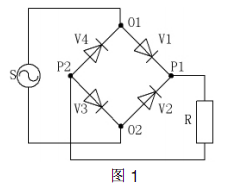
\includegraphics[width=0.3\textwidth]{.images/FullRectification.png}
        \caption{Full Rectification}
    \end{figure}

    \subsection{Smoothing}

    \begin{displaymath}
        I = {I_0}e^{-\frac{t}{RC}}
    \end{displaymath}

    \subsection{Transformer}

    \subsubsection{Principle}
    \begin{itemize}
        \item In primary coil, an AC producing a changing flux in iron core,
        \item flux links to the secondary coil,
        \item in secondary coil, changing flux induced an e.m.f.
    \end{itemize}

    \subsubsection{Function of iron core}
    \begin{itemize}
        \item Prevent flux loses.
    \end{itemize}

    \subsubsection{Why $V_p$ and $V_s$ not in phase}
    \begin{itemize}
        \item $V_p$ is proportional to changing magnetic flux,
        \item $V_s$ is proportional to the rate of change of flux.
    \end{itemize}


    \section{Quantum Physics}

    \subsection{Momentum and energy}
    \begin{displaymath}
        \lambda = \frac{h}{\sqrt{2mQV}}
    \end{displaymath}
\end{document}